% Created 2025-01-11 Sat 07:55
% Intended LaTeX compiler: pdflatex
\documentclass[11pt]{article}
\usepackage[utf8]{inputenc}
\usepackage[T1]{fontenc}
\usepackage{graphicx}
\usepackage{longtable}
\usepackage{wrapfig}
\usepackage{rotating}
\usepackage[normalem]{ulem}
\usepackage{amsmath}
\usepackage{amssymb}
\usepackage{capt-of}
\usepackage{hyperref}
\date{\today}
\title{}
\hypersetup{
 pdfauthor={},
 pdftitle={},
 pdfkeywords={},
 pdfsubject={},
 pdfcreator={Emacs 29.4 (Org mode 9.7.12)}, 
 pdflang={English}}
\begin{document}

\tableofcontents

\documentclass[11pt]{article}
\usepackage[utf8]{inputenc}
\usepackage[T1]{fontenc}
\usepackage{graphicx}
\usepackage{longtable}
\usepackage{wrapfig}
\usepackage{rotating}
\usepackage[normalem]{ulem}
\usepackage{amsmath}
\usepackage{amssymb}
\usepackage{capt-of}
\usepackage{hyperref}
\usepackage{tikz}
\usepackage[paperwidth=14.58in, paperheight=10.42in, margin=0.1in]{geometry}
\pagestyle{empty}
\date{}
\title{Neural Network Diagram}
\hypersetup\{
 pdfauthor=\{\},
 pdftitle=\{Neural Network Diagram\},
 pdfkeywords=\{\},
 pdfsubject=\{\},
 pdfcreator=\{Emacs 29.4 (Org mode 9.7.12)\}, 
 pdflang=\{English\}\}
\begin{document}

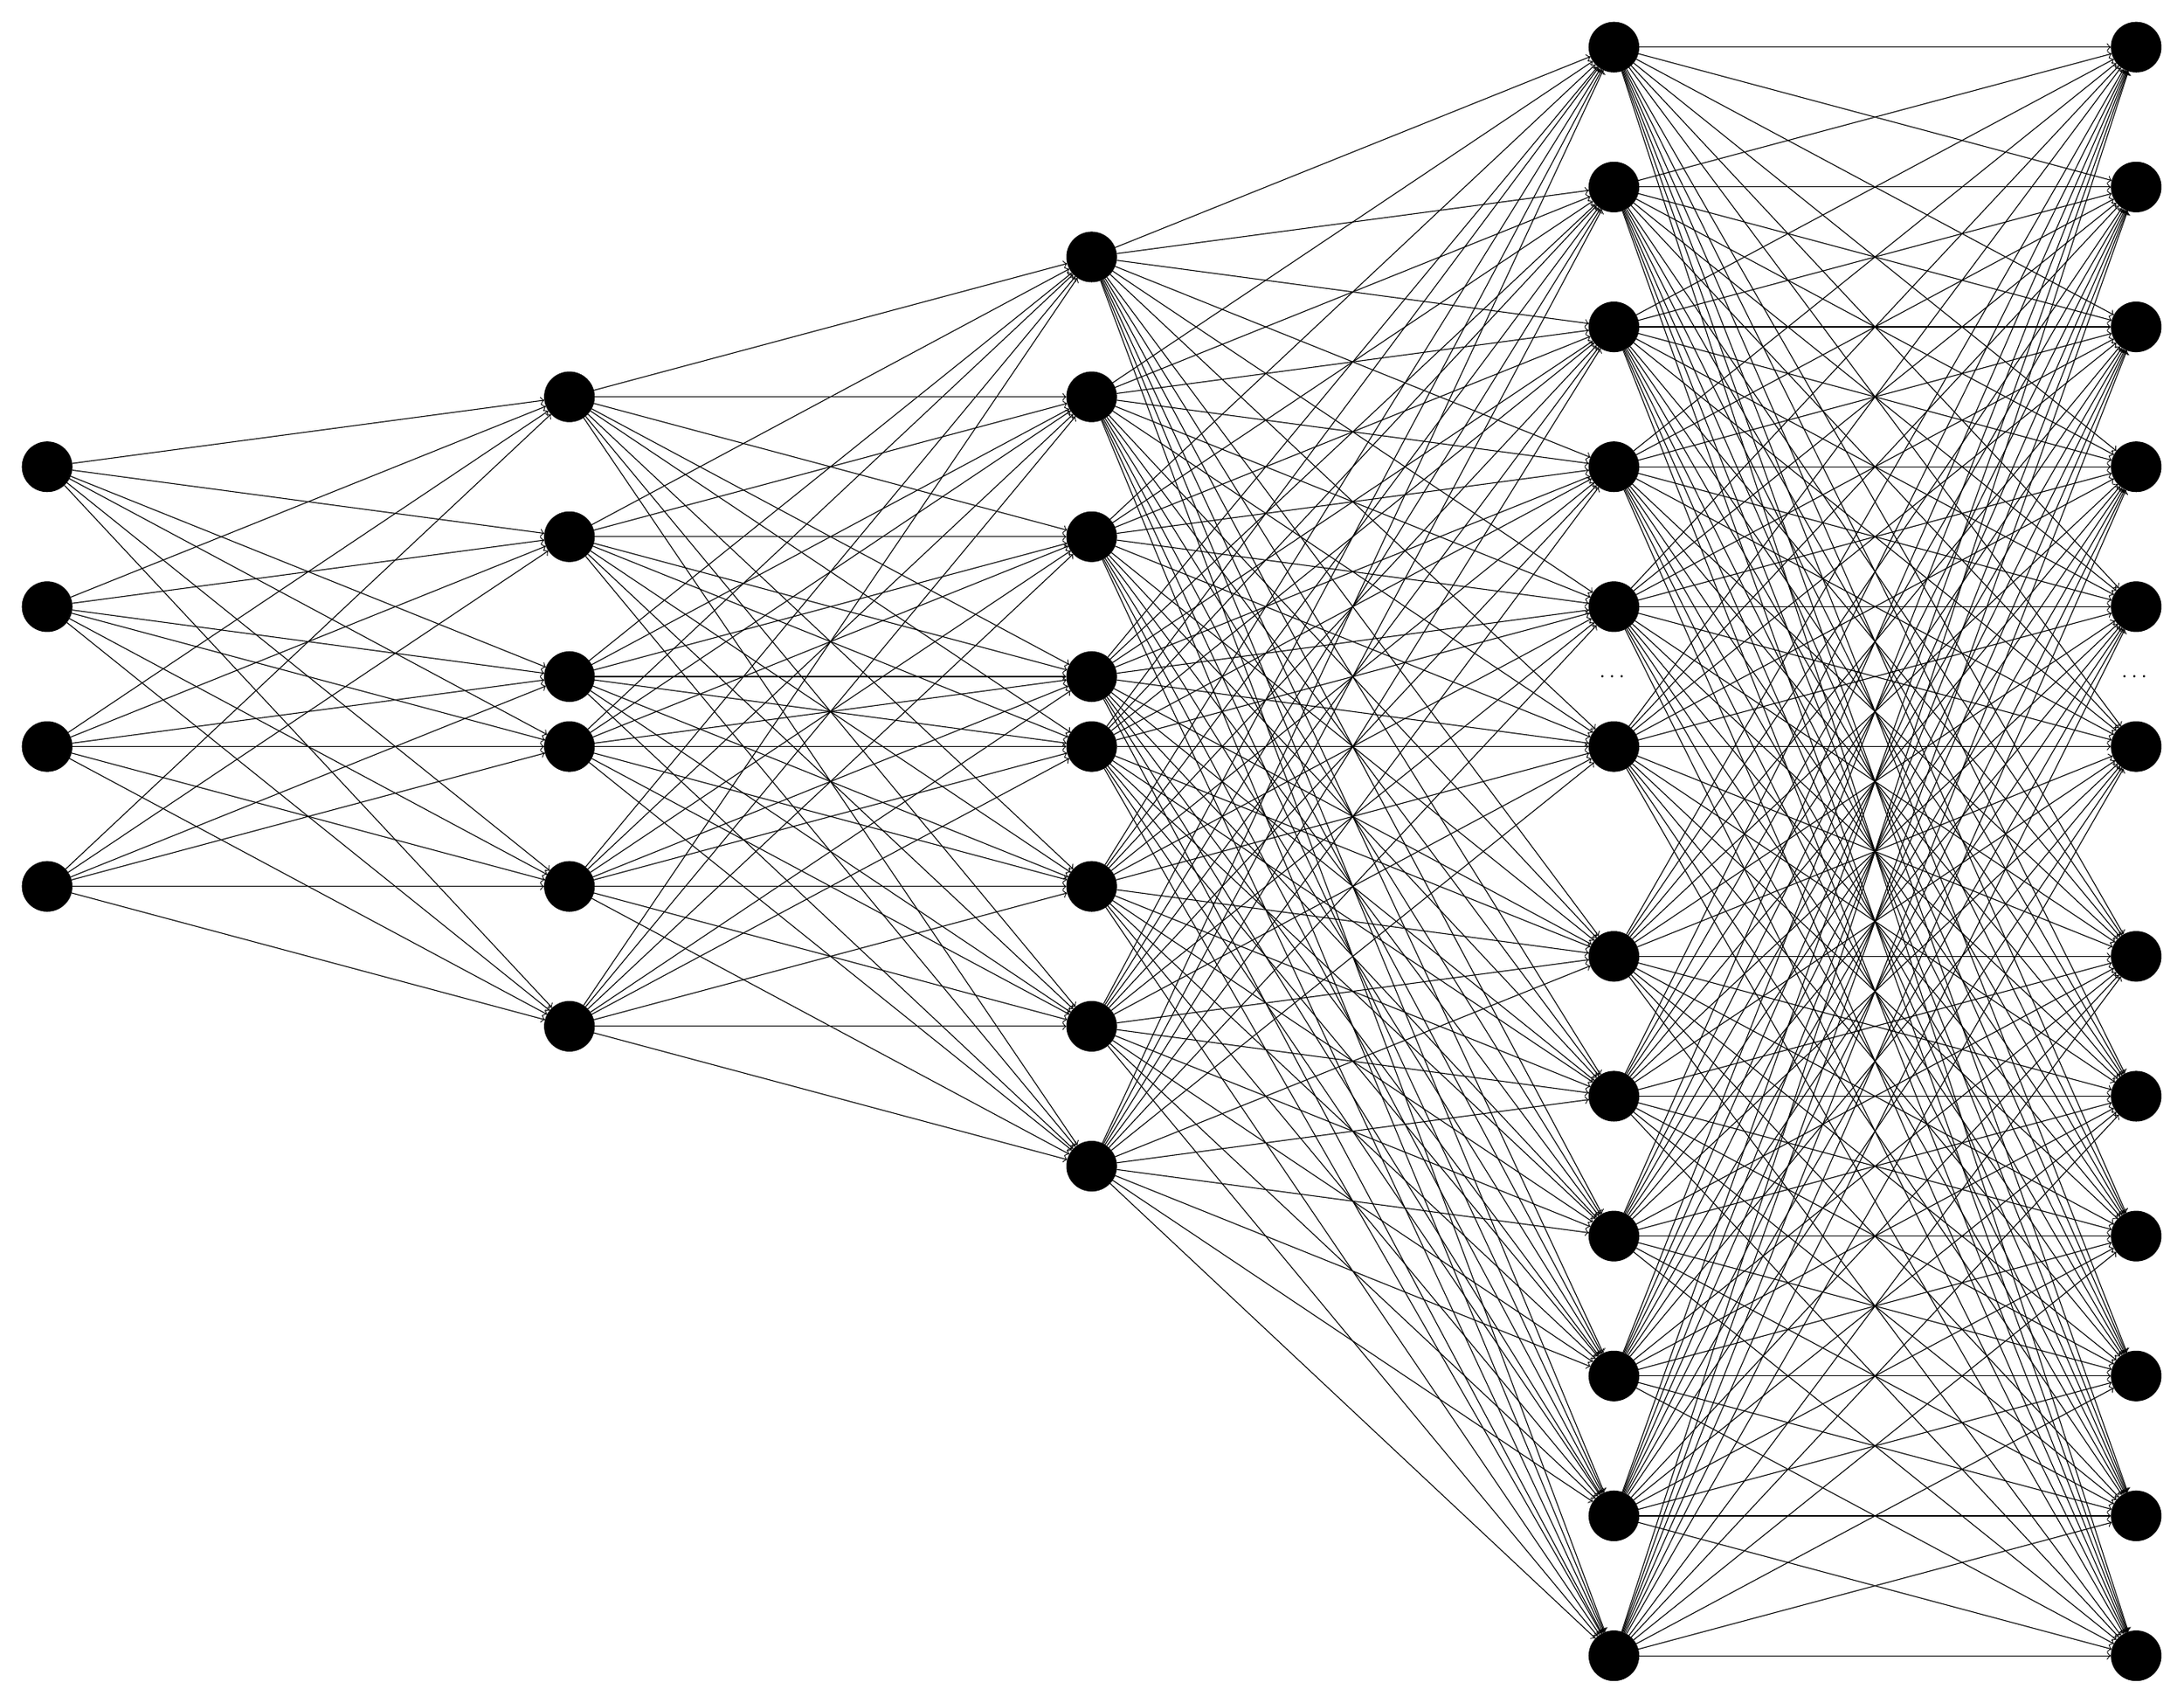
\begin{tikzpicture}[every node/.style={circle, draw,fill=black, minimum size=0.8cm}, node distance=2cm]

% Define a variable for spacing
\def\spacing{2.25}
\def\hspacing{2.8}

% Input layer (4 neurons)
\foreach \i in {1,...,4} {
    \node (input\i) at (\hspacing*0, {0 - \spacing * (\i-1)}) {};
}

% First hidden layer (6 neurons + "...")
\foreach \i in {1,...,3} {
    \node (h1_\i) at (\hspacing*3, {0.5*\spacing - \spacing * (\i-1)}) {};
}
\node[draw=none, fill=none] (h1_dot) at (\hspacing*3, {-1.5*\spacing}) {…};
\foreach \i in {4,...,6} {
    \node (h1_\i) at (\hspacing*3, {-2*\spacing - \spacing * (\i-4)}) {};
}

% Second hidden layer (8 neurons + "...")
\foreach \i in {1,...,4} {
    \node (h2_\i) at (\hspacing*6, {1.5*\spacing - \spacing * (\i-1)}) {};
}
\node[draw=none, fill=none] (h2_dot) at (\hspacing*6, {-0.5*\spacing}) {…};
\foreach \i in {5,...,8} {
    \node (h2_\i) at (\hspacing*6, {-2*\spacing - \spacing * (\i-5)}) {};
}

% Third hidden layer (12 neurons + "...")
\foreach \i in {1,...,6} {
    \node (h3_\i) at (\hspacing*9, {3*\spacing - \spacing * (\i-1)}) {};
}
\node[draw=none, fill=none] (h3_dot) at (\hspacing*9, {-1.5*\spacing}) {…};
\foreach \i in {7,...,12} {
    \node (h3_\i) at (\hspacing*9, {-3.5*\spacing - \spacing * (\i-7)}) {};
}

% Fourth hidden layer (12 neurons + "...")
\foreach \i in {1,...,6} {
    \node (h4_\i) at (\hspacing*12, {3*\spacing - \spacing * (\i-1)}) {};
}
\node[draw=none, fill=none] (h4_dot) at (\hspacing*12, {-1.5*\spacing}) {…};
\foreach \i in {7,...,12} {
    \node (h4_\i) at (\hspacing*12, {-3.5*\spacing - \spacing * (\i-7)}) {};
}

% Connections from input to first hidden layer
\foreach \i in {1,...,4} {
    \foreach \j in {1,...,3} {
        \draw[->] (input\i) -- (h1_\j);
    }
    \foreach \j in {4,...,6} {
        \draw[->] (input\i) -- (h1_\j);
    }
}

% Connections from first hidden to second hidden layer
\foreach \i in {1,...,3} {
    \foreach \j in {1,...,4} {
        \draw[->] (h1_\i) -- (h2_\j);
    }
    \foreach \j in {5,...,8} {
        \draw[->] (h1_\i) -- (h2_\j);
    }
}

\foreach \i in {4,...,6} {
    \foreach \j in {1,...,4} {
        \draw[->] (h1_\i) -- (h2_\j);
    }
    \foreach \j in {5,...,8} {
        \draw[->] (h1_\i) -- (h2_\j);
    }
}

% Connections from second hidden to third hidden layer
\foreach \i in {1,...,4} {
    \foreach \j in {1,...,6} {
        \draw[->] (h2_\i) -- (h3_\j);
    }
    \foreach \j in {7,...,12} {
        \draw[->] (h2_\i) -- (h3_\j);
    }
}
\foreach \i in {5,...,8} {
    \foreach \j in {1,...,6} {
        \draw[->] (h2_\i) -- (h3_\j);
    }
    \foreach \j in {7,...,12} {
        \draw[->] (h2_\i) -- (h3_\j);
    }
}

% Connections from third hidden to fourth hidden layer
\foreach \i in {1,...,6} {
    \foreach \j in {1,...,6} {
        \draw[->] (h3_\i) -- (h4_\j);
    }
    \foreach \j in {7,...,12} {
        \draw[->] (h3_\i) -- (h4_\j);
    }
}
\foreach \i in {7,...,12} {
    \foreach \j in {1,...,6} {
        \draw[->] (h3_\i) -- (h4_\j);
    }
    \foreach \j in {7,...,12} {
        \draw[->] (h3_\i) -- (h4_\j);
    }
}

\end{tikzpicture}
\end{document}
\end{document}
